%!TeX root=../houndtop.tex
\chapter{A Retrospection}

\lettrine[lines=4]{I}{t} was the end of November and Holmes and I sat, upon a raw and foggy night, on either side of a blazing fire in our sitting-room in Baker Street. Since the tragic upshot of our visit to Devonshire he had been engaged in two affairs of the utmost importance, in the first of which he had exposed the atrocious conduct of Colonel Upwood in connection with the famous card scandal of the Nonpareil Club, while in the second he had defended the unfortunate Mme. Montpensier from the charge of murder which hung over her in connection with the death of her step-daughter, Mlle Carére, the young lady who, as it will be re\-mem\-bered, was found six months later alive and married in New York. My friend was in excellent spirits over the success which had attended a succession of difficult and important cases, so that I was able to induce him to discuss the details of the Baskerville mystery. I had waited patiently for the opportunity, for I was aware that he would never permit cases to overlap, and that his clear and logical mind would not be drawn from its present work to dwell upon memories of the past. Sir Henry and Dr Mortimer were, however, in London, on their way to that long voyage which had been recommended for the restoration of his shattered nerves. They had called upon us that very afternoon, so that it was natural that the subject should come up for discussion.

%\begin{figure}[tbph]
%\centering
%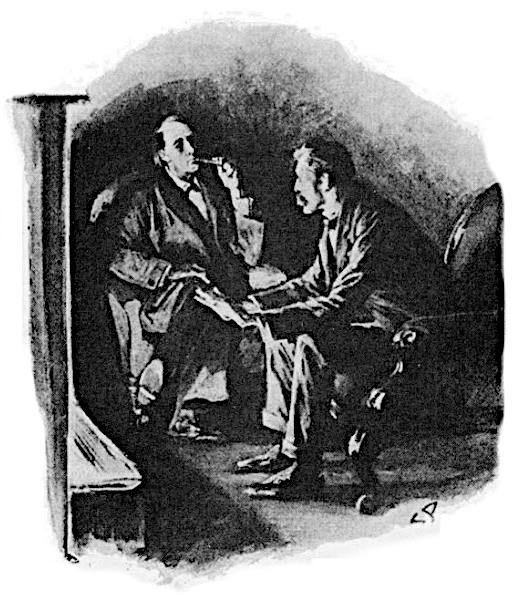
\includegraphics[width=0.7\linewidth]{15_retro}
%\caption*{A retrospection}
%\end{figure}

%\begin{wrapfigure}{O}{0.5\textwidth}
%\centering
%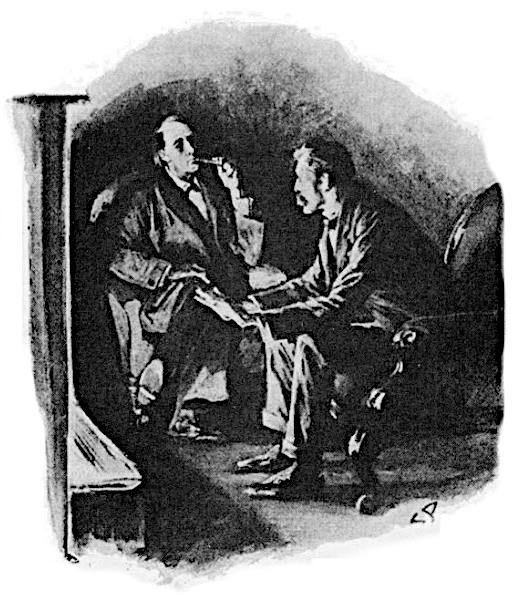
\includegraphics[width=0.5\linewidth]{15_retro}
%\caption*{A retrospection}
%\end{wrapfigure}

»The whole course of events,« said Holmes, »from the point of view of the man who called himself Stapleton was simple and direct, although to us, who had no means in the beginning of knowing the motives of his actions and could only learn part of the facts, it all appeared exceedingly complex. I have had the advantage of two conversations with Mrs Stapleton, and the case has now been so entirely cleared up that I am not aware that there is anything which has remained a secret to us. You will find a few notes upon the matter under the heading B in my indexed list of cases.«

»Perhaps you would kindly give me a sketch of the course of events from memory.«

»Certainly, though I cannot guarantee that I carry all the facts in my mind. Intense mental concentration has a curious way of blotting out what has passed. The barrister who has his case at his fingers' ends, and is able to argue with an expert upon his own subject finds that a week or two of the courts will drive it all out of his head once more. So each of my cases displaces the last, and Mlle Carére has blurred my recollection of Baskerville Hall. To-morrow some other little problem may be submitted to my notice which will in turn dispossess the fair French lady and the infamous Upwood. So far as the case of the Hound goes, however, I will give you the course of events as nearly as I can, and you will suggest anything which I may have forgotten.«

»My inquiries show beyond all question that the family portrait did not lie, and that this fellow was indeed a Baskerville. He was a son of that Rodger Baskerville, the younger brother of Sir Charles, who fled with a sinister reputation to South America, where he was said to have died unmarried. He did, as a matter of fact, marry, and had one child, this fellow, whose real name is the same as his father's. He married Beryl Garcia, one of the beauties of Costa Rica, and, having purloined a considerable sum of public money, he changed his name to Vandeleur and fled to England, where he established a school in the east of Yorkshire. His reason for attempting this special line of business was that he had struck up an acquaintance with a consumptive tutor upon the voyage home, and that he had used this man's ability to make the undertaking a success. Fraser, the tutor, died however, and the school which had begun well sank from disrepute into infamy. The Vandeleurs found it convenient to change their name to Stapleton, and he brought the remains of his fortune, his schemes for the future, and his taste for entomology to the south of England. I learned at the British Museum that he was a recognized authority upon the subject, and that the name of Vandeleur has been permanently attached to a certain moth which he had, in his Yorkshire days, been the first to describe.«

»We now come to that portion of his life which has proved to be of such intense interest to us. The fellow had evidently made inquiry and found that only two lives intervened between him and a valuable estate. When he went to Devonshire his plans were, I believe, exceedingly hazy, but that he meant mischief from the first is evident from the way in which he took his wife with him in the character of his sister. The idea of using her as a decoy was clearly already in his mind, though he may not have been certain how the details of his plot were to be arranged. He meant in the end to have the estate, and he was ready to use any tool or run any risk for that end. His first act was to establish himself as near to his ancestral home as he could, and his second was to cultivate a friendship with Sir Charles Baskerville and with the neighbours.«

»The baronet himself told him about the family hound, and so prepared the way for his own death. Stapleton, as I will continue to call him, knew that the old man's heart was weak and that a shock would kill him. So much he had learned from Dr Mortimer. He had heard also that Sir Charles was superstitious and had taken this grim legend very seriously. His ingenious mind instantly suggested a way by which the baronet could be done to death, and yet it would be hardly possible to bring home the guilt to the real murderer.«

»Having conceived the idea he proceeded to carry it out with considerable finesse. An ordinary schemer would have been content to work with a savage hound. The use of artificial means to make the creature diabolical was a flash of genius upon his part. The dog he bought in London from Ross and Mangles, the dealers in Fulham Road. It was the strongest and most savage in their possession. He brought it down by the North Devon line and walked a great distance over the moor so as to get it home without exciting any remarks. He had already on his insect hunts learned to penetrate the Grimpen Mire, and so had found a safe hiding-place for the creature. Here he kennelled it and waited his chance.«

»But it was some time coming. The old gentleman could not be decoyed outside of his grounds at night. Several times Stapleton lurked about with his hound, but without avail. It was during these fruitless quests that he, or rather his ally, was seen by peasants, and that the legend of the demon dog received a new confirmation. He had hoped that his wife might lure Sir Charles to his ruin, but here she proved unexpectedly independent. She would not endeavour to entangle the old gentleman in a sentimental attachment which might deliver him over to his enemy. Threats and even, I am sorry to say, blows refused to move her. She would have nothing to do with it, and for a time Stapleton was at a deadlock.«

»He found a way out of his difficulties through the chance that Sir Charles, who had conceived a friendship for him, made him the minister of his charity in the case of this unfortunate woman, Mrs Laura Lyons. By representing himself as a single man he acquired complete influence over her, and he gave her to understand that in the event of her obtaining a divorce from her husband he would marry her. His plans were suddenly brought to a head by his knowledge that Sir Charles was about to leave the Hall on the advice of Dr Mortimer, with whose opinion he himself pretended to coincide. He must act at once, or his victim might get beyond his power. He therefore put pressure upon Mrs Lyons to write this letter, imploring the old man to give her an interview on the evening before his departure for London. He then, by a specious argument, prevented her from going, and so had the chance for which he had waited.«

»Driving back in the evening from Coombe Tracey he was in time to get his hound, to treat it with his infernal paint, and to bring the beast round to the gate at which he had reason to expect that he would find the old gentleman waiting. The dog, incited by its master, sprang over the wicket-gate and pursued the unfortunate baronet, who fled screaming down the Yew Alley. In that gloomy tunnel it must indeed have been a dreadful sight to see that huge black creature, with its flaming jaws and blazing eyes, bounding after its victim. He fell dead at the end of the alley from heart disease and terror. The hound had kept upon the grassy border while the baronet had run down the path, so that no track but the man's was visible. On seeing him lying still the creature had probably approached to sniff at him, but finding him dead had turned away again. It was then that it left the print which was actually observed by Dr Mortimer. The hound was called off and hurried away to its lair in the Grimpen Mire, and a mystery was left which puzzled the authorities, alarmed the country-side, and finally brought the case within the scope of our observation.«

»So much for the death of Sir Charles Baskerville. You perceive the devilish cunning of it, for really it would be almost impossible to make a case against the real murderer. His only accomplice was one who could never give him away, and the grotesque, inconceivable nature of the device only served to make it more effective. Both of the women concerned in the case, Mrs Stapleton and Mrs Laura Lyons, were left with a strong suspicion against Stapleton. Mrs Stapleton knew that he had designs upon the old man, and also of the existence of the hound. Mrs Lyons knew neither of these things, but had been impressed by the death occurring at the time of an uncancelled appointment which was only known to him. However, both of them were under his influence, and he had nothing to fear from them. The first half of his task was successfully accomplished but the more difficult still remained.«

»It is possible that Stapleton did not know of the existence of an heir in Canada. In any case he would very soon learn it from his friend Dr Mortimer, and he was told by the latter all details about the arrival of Henry Baskerville. Stapleton's first idea was that this young stranger from Canada might possibly be done to death in London without coming down to Devonshire at all. He distrusted his wife ever since she had refused to help him in laying a trap for the old man, and he dared not leave her long out of his sight for fear he should lose his influence over her. It was for this reason that he took her to London with him. They lodged, I find, at the Mexborough Private Hotel, in Craven Street, which was actually one of those called upon by my agent in search of evidence. Here he kept his wife imprisoned in her room while he, disguised in a beard, followed Dr Mortimer to Baker Street and afterwards to the station and to the Northumberland Hotel. His wife had some inkling of his plans; but she had such a fear of her husband—a fear founded upon brutal ill-treatment—that she dare not write to warn the man whom she knew to be in danger. If the letter should fall into Stapleton's hands her own life would not be safe. Eventually, as we know, she adopted the expedient of cutting out the words which would form the message, and addressing the letter in a disguised hand. It reached the baronet, and gave him the first warning of his danger.«

»It was very essential for Stapleton to get some article of Sir Henry's attire so that, in case he was driven to use the dog, he might always have the means of setting him upon his track. With characteristic promptness and audacity he set about this at once, and we cannot doubt that the boots or chamber-maid of the hotel was well bribed to help him in his design. By chance, however, the first boot which was procured for him was a new one and, therefore, useless for his purpose. He then had it returned and obtained another—a most instructive incident, since it proved conclusively to my mind that we were dealing with a real hound, as no other supposition could explain this anxiety to obtain an old boot and this indifference to a new one. The more \textit{outré} and grotesque an incident is the more carefully it deserves to be examined, and the very point which appears to complicate a case is, when duly considered and scientifically handled, the one which is most likely to elucidate it.«

»Then we had the visit from our friends next morning, shadowed always by Stapleton in the cab. From his knowledge of our rooms and of my appearance, as well as from his general conduct, I am inclined to think that Stapleton's career of crime has been by no means limited to this single Baskerville affair. It is suggestive that during the last three years there have been four considerable burglaries in the West Country, for none of which was any criminal ever arrested. The last of these, at Folkestone Court, in May, was remarkable for the cold-blooded pistolling of the page, who surprised the masked and solitary burglar. I cannot doubt that Stapleton recruited his waning resources in this fashion, and that for years he has been a desperate and dangerous man.«

»We had an example of his readiness of resource that morning when he got away from us so successfully, and also of his audacity in sending back my own name to me through the cabman. From that moment he understood that I had taken over the case in London, and that therefore there was no chance for him there. He returned to Dartmoor and awaited the arrival of the baronet.«

»One moment!« said I. »You have, no doubt, described the sequence of events correctly, but there is one point which you have left unexplained. What became of the hound when its master was in London?«

»I have given some attention to this matter and it is undoubtedly of importance. There can be no question that Stapleton had a confidant, though it is unlikely that he ever placed himself in his power by sharing all his plans with him. There was an old manservant at Merripit House, whose name was Anthony. His connection with the Stapletons can be traced for several years, as far back as the schoolmastering days, so that he must have been aware that his master and mistress were really husband and wife. This man has disappeared and has escaped from the country. It is suggestive that Anthony is not a common name in England, while Antonio is so in all Spanish or Spanish-American countries. The man, like Mrs Stapleton herself, spoke good English, but with a curious lisping accent. I have myself seen this old man cross the Grimpen Mire by the path which Stapleton had marked out. It is very probable, therefore, that in the absence of his master it was he who cared for the hound, though he may never have known the purpose for which the beast was used.«

»The Stapletons then went down to Devonshire, whither they were soon followed by Sir Henry and you. One word now as to how I stood myself at that time. It may possibly recur to your memory that when I examined the paper upon which the printed words were fastened I made a close inspection for the water-mark. In doing so I held it within a few inches of my eyes, and was conscious of a faint smell of the scent known as white jessamine. There are seventy-five perfumes, which it is very necessary that a criminal expert should be able to distinguish from each other, and cases have more than once within my own experience depended upon their prompt recognition. The scent suggested the presence of a lady, and already my thoughts began to turn towards the Stapletons. Thus I had made certain of the hound, and had guessed at the criminal before ever we went to the West Country.«

»It was my game to watch Stapleton. It was evident, however, that I could not do this if I were with you, since he would be keenly on his guard. I deceived everybody, therefore, yourself included, and I came down secretly when I was supposed to be in London. My hardships were not so great as you imagined, though such trifling details must never interfere with the investigation of a case. I stayed for the most part at Coombe Tracey, and only used the hut upon the moor when it was necessary to be near the scene of action. Cartwright had come down with me, and in his disguise as a country boy he was of great assistance to me. I was dependent upon him for food and clean linen. When I was watching Stapleton, Cartwright was frequently watching you, so that I was able to keep my hand upon all the strings.«

»I have already told you that your reports reached me rapidly, being forwarded instantly from Baker Street to Coombe Tracey. They were of great service to me, and especially that one incidentally truthful piece of biography of Stapleton's. I was able to establish the identity of the man and the woman and knew at last exactly how I stood. The case had been considerably complicated through the incident of the escaped convict and the relations between him and the Barrymores. This also you cleared up in a very effective way, though I had already come to the same conclusions from my own observations.«

»By the time that you discovered me upon the moor I had a complete knowledge of the whole business, but I had not a case which could go to a jury. Even Stapleton's attempt upon Sir Henry that night which ended in the death of the unfortunate convict did not help us much in proving murder against our man. There seemed to be no alternative but to catch him red-handed, and to do so we had to use Sir Henry, alone and apparently unprotected, as a bait. We did so, and at the cost of a severe shock to our client we succeeded in completing our case and driving Stapleton to his destruction. That Sir Henry should have been exposed to this is, I must confess, a reproach to my management of the case, but we had no means of foreseeing the terrible and paralyzing spectacle which the beast presented, nor could we predict the fog which enabled him to burst upon us at such short notice. We succeeded in our object at a cost which both the specialist and Dr Mortimer assure me will be a temporary one. A long journey may enable our friend to recover not only from his shattered nerves but also from his wounded feelings. His love for the lady was deep and sincere, and to him the saddest part of all this black business was that he should have been deceived by her.«

»It only remains to indicate the part which she had played throughout. There can be no doubt that Stapleton exercised an influence over her which may have been love or may have been fear, or very possibly both, since they are by no means incompatible emotions. It was, at least, absolutely effective. At his command she consented to pass as his sister, though he found the limits of his power over her when he endeavoured to make her the direct accessory to murder. She was ready to warn Sir Henry so far as she could without implicating her husband, and again and again she tried to do so. Stapleton himself seems to have been capable of jealousy, and when he saw the baronet paying court to the lady, even though it was part of his own plan, still he could not help interrupting with a passionate outburst which revealed the fiery soul which his self-contained manner so cleverly concealed. By encouraging the intimacy he made it certain that Sir Henry would frequently come to Merripit House and that he would sooner or later get the opportunity which he desired. On the day of the crisis, however, his wife turned suddenly against him. She had learned something of the death of the convict, and she knew that the hound was being kept in the out-house on the evening that Sir Henry was coming to dinner. She taxed her husband with his intended crime, and a furious scene followed, in which he showed her for the first time that she had a rival in his love. Her fidelity turned in an instant to bitter hatred and he saw that she would betray him. He tied her up, therefore, that she might have no chance of warning Sir Henry, and he hoped, no doubt, that when the whole country-side put down the baronet's death to the curse of his family, as they certainly would do, he could win his wife back to accept an accomplished fact and to keep silent upon what she knew. In this I fancy that in any case he made a miscalculation, and that, if we had not been there, his doom would none the less have been sealed. A woman of Spanish blood does not condone such an injury so lightly. And now, my dear Watson, without referring to my notes, I cannot give you a more detailed account of this curious case. I do not know that anything essential has been left unexplained.«

»He could not hope to frighten Sir Henry to death as he had done the old uncle with his bogie hound.«

»The beast was savage and half-starved. If its appearance did not frighten its victim to death, at least it would paralyse the resistance which might be offered.«

»No doubt. There only remains one difficulty. If Stapleton came into the succession, how could he explain the fact that he, the heir, had been living unannounced under another name so close to the property? How could he claim it without causing suspicion and inquiry?«

%»It is a formidable difficulty, and I fear that you ask too much when you expect me to solve it. The past and the present are within the field of my inquiry, but what a man may do in the future is a hard question to answer. Mrs Stapleton had heard her husband discuss the problem on several occasions. There were three possible courses. He might claim the property from South America, establish his identity before the British authorities there and so obtain the fortune without ever coming to England at all; or he might adopt an elaborate disguise during the short time that he need be in London; or, again, he might furnish an accomplice with the proofs and papers, putting him in as heir, and retaining a claim upon some proportion of his income. We cannot doubt from what we know of him that he would have found some way out of the difficulty. And now, my dear Watson, we have had some weeks of severe work, and for one evening, I think, we may turn our thoughts into more pleasant channels. I have a box for \textit{Les Huguenots}\footnote{Opera by Giacomo Meyerbeer (1791-1864), premiered in 1836.}. Have you heard the De Reszkes\footnote{Jean (1850-1904; tenor), Édouard (1853-1917; bass), and Josephine (1855-1891; soprano) de Reszke, sibling opera singers.}? Might I trouble you then to be ready in half an hour, and we can stop at Marcini's for a little dinner on the way?«

»It is a formidable difficulty, and I fear that you ask too much when you expect me to solve it. The past and the present are within the field of my inquiry, but what a man may do in the future is a hard question to answer. Mrs Stapleton had heard her husband discuss the problem on several occasions. There were three possible courses. He might claim the property from South America, establish his identity before the British authorities there and so obtain the fortune without ever coming to England at all; or he might adopt an elaborate disguise during the short time that he need be in London; or, again, he might furnish an accomplice with the proofs and papers, putting him in as heir, and retaining a claim upon some proportion of his income. We cannot doubt from what we know of him that he would have found some way out of the difficulty. And now, my dear Watson, we have had some weeks of severe work, and for one evening, I think, we may turn our thoughts into more pleasant channels. I have a box for \textit{Les Huguenots}. Have you heard the De Reszkes? Might I trouble you then to be ready in half an hour, and we can stop at Marcini's for a little dinner on the way?«




 
\makeatletter
\@ifclasswith{scrbook}{a5paper}
{%
}{%
	\centering
	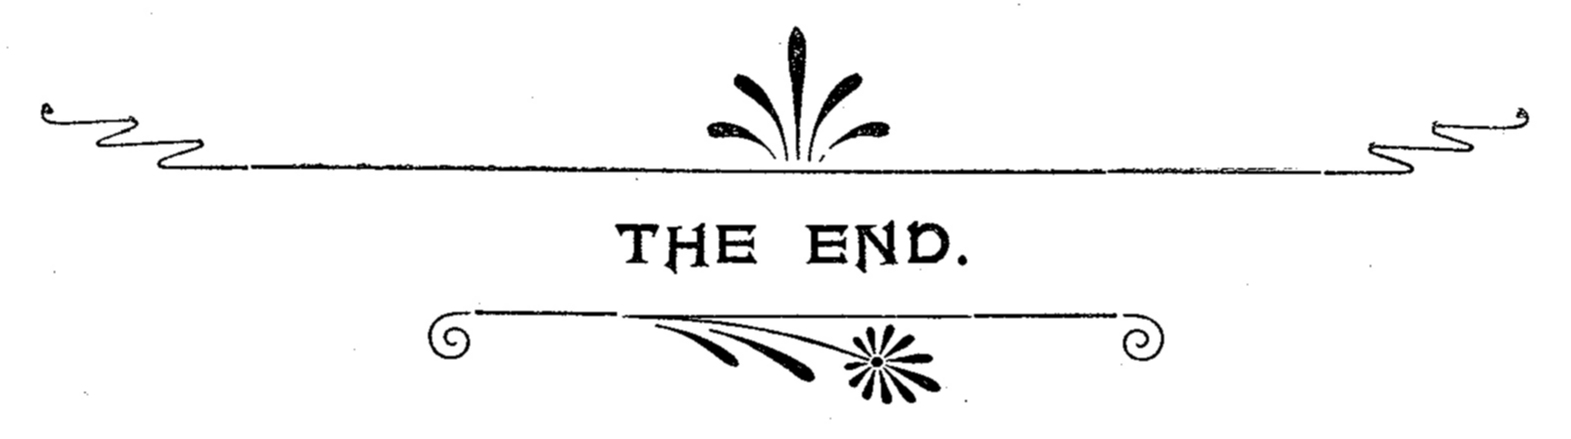
\includegraphics[width=0.9\linewidth]{theend}
	\thispagestyle{headings}
%	\clearpage
}

\makeatother
   